
\documentclass[11pt]{article}

\marginparwidth 0.2in 
\oddsidemargin 0.1in 
\evensidemargin 0.1in 
\marginparsep 0.1in
\topmargin 0.1in 
\textwidth 6.5in \textheight 8 in

\usepackage{hyperref}  
\usepackage{listings}
\usepackage{array}
\usepackage{multirow}
\usepackage{attachfile}
\usepackage{lscape}
\usepackage{graphicx}
\usepackage{etoolbox}
\usepackage[usenames,dvipsnames]{xcolor}
\usepackage{transparent}

\makeatletter
\patchcmd{\@maketitle}{\vskip 2em}{\vspace*{-3cm}}{}{}
\makeatother

\author{İbrahim Burak Tanrıkulu, 21827852}
\title{BBM434 Gömülü Sistemler Lab.\\Deney 1}

\lstset {language=C, tabsize=4, backgroundcolor =  \transparent{.3}\color{gray}}
\newcommand\tab[1][1cm]{\hspace*{#1}}

\begin{document}
\maketitle

\section{Switch Bouncing nedir, nasıl önlenir?}
Bir butona bastığımızda, bir anahtarı açıp kapattığımızda bunların içerisindeki metaller birleşerek akım iletilir. Ama bu metallerin birbirine en yakın oldukları zamanda elektriğin hava yoluyla iletilmesi sonucu (elektrik arkı) sanki birden fazla kez butona basmış gibi algılanabilir. 1ms gibi küçük bir süre içerisinde 10-100 kez bu akım oluşur.\\
Bu durumu engellemenin hem donanımsal, hem de yazılımsal yolları vardır. Biz donanımsal çözümlerden biri olan "sayma" yöntemini kullanacağız.

\section{Kullanacağımız devre}
Switch Bounce olayını gösterebilmek için push button kullanacağız. Eğer debouncing yapmadan buton ile LED yakarsanız bazen LED'in yanmadığını, hızlı yanıp söndüğünü görebilirsiniz. Fakat debounce yaptığınızda bu sorunlarla karşılaşmayacaksınız.\\
Bildiğiniz gibi Arduino Uno'nun 13. pini dahili LED'e bağlıdır. Biz de bu dahili LED'i kullanacağız. Buton girdisi için herhangi pini kullanabilirsiniz. Ben 7. pini kullandım. Devremiz şu şekilde:

\begin{minipage}{0.95\textwidth}
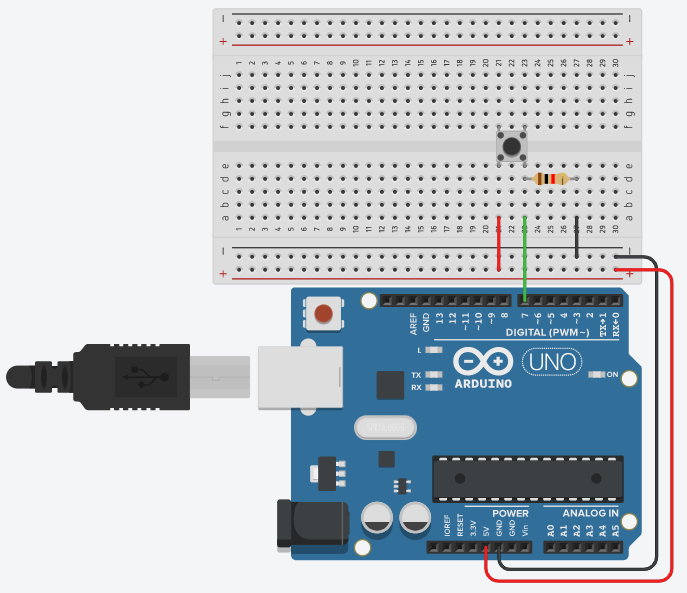
\includegraphics[width=12cm]{Debouncing.png}
\centering
\end{minipage}

\section{Yazılımla Switch Debouncing}
Yazılımımızda birkaç değişken kullanacağız:
\begin{lstlisting}
int counter = 0;       	  // bu degisken uzerinden sayacagiz
int reading;           	  // okudugumuz deger
int current_state = LOW;  // mevcut durum
int debounce_count = 10;  // bu sayiya kadar sayabilmeliyiz
\end{lstlisting}
Programımız bir döngü ile sürekli devam edecek.\\
İlk önce 7. pinden sinyali okuyoruz.
\begin{lstlisting}
reading = digitalRead(inPin);
\end{lstlisting}
Eğer aynı değeri okuyorsak sayımımızı düşürüyoruz. (Tabi eğer zaten sıfır değilse)
\begin{lstlisting}
if(reading == current_state && counter > 0)
{
	counter--;
}
\end{lstlisting}
Eğer farklı bir değer okuyorsak, sayımımızı arttırıyoruz.
\begin{lstlisting}
if(reading != current_state)
{
	counter++; 
}
\end{lstlisting}
Eğer istenilen sayıya kadar saymışsak, artık emin olabiliriz. LED'i yakma/söndürme zamanı gelmiş.
\begin{lstlisting}
if(counter >= debounce_count)
{
	counter = 0;
	current_state = reading;
	digitalWrite(outPin, current_state);
}
\end{lstlisting}
Yazdığımız koda buradan ulaşabilirsiniz: \attachfile{debouncing.ino}
\newpage
\section{Deney}
Yazılımımız hazır, tasarımı da yaptık. Gerçek hayatta deneyelim o zaman. Arduino IDE ile kodumuzu yazıp USB bağlantısıyla Arduino Uno'ya yüklüyoruz. Daha sonrasında devremizi kurup denemeye başlayabiliriz.\\~\\
\begin{minipage}{0.5\textwidth}
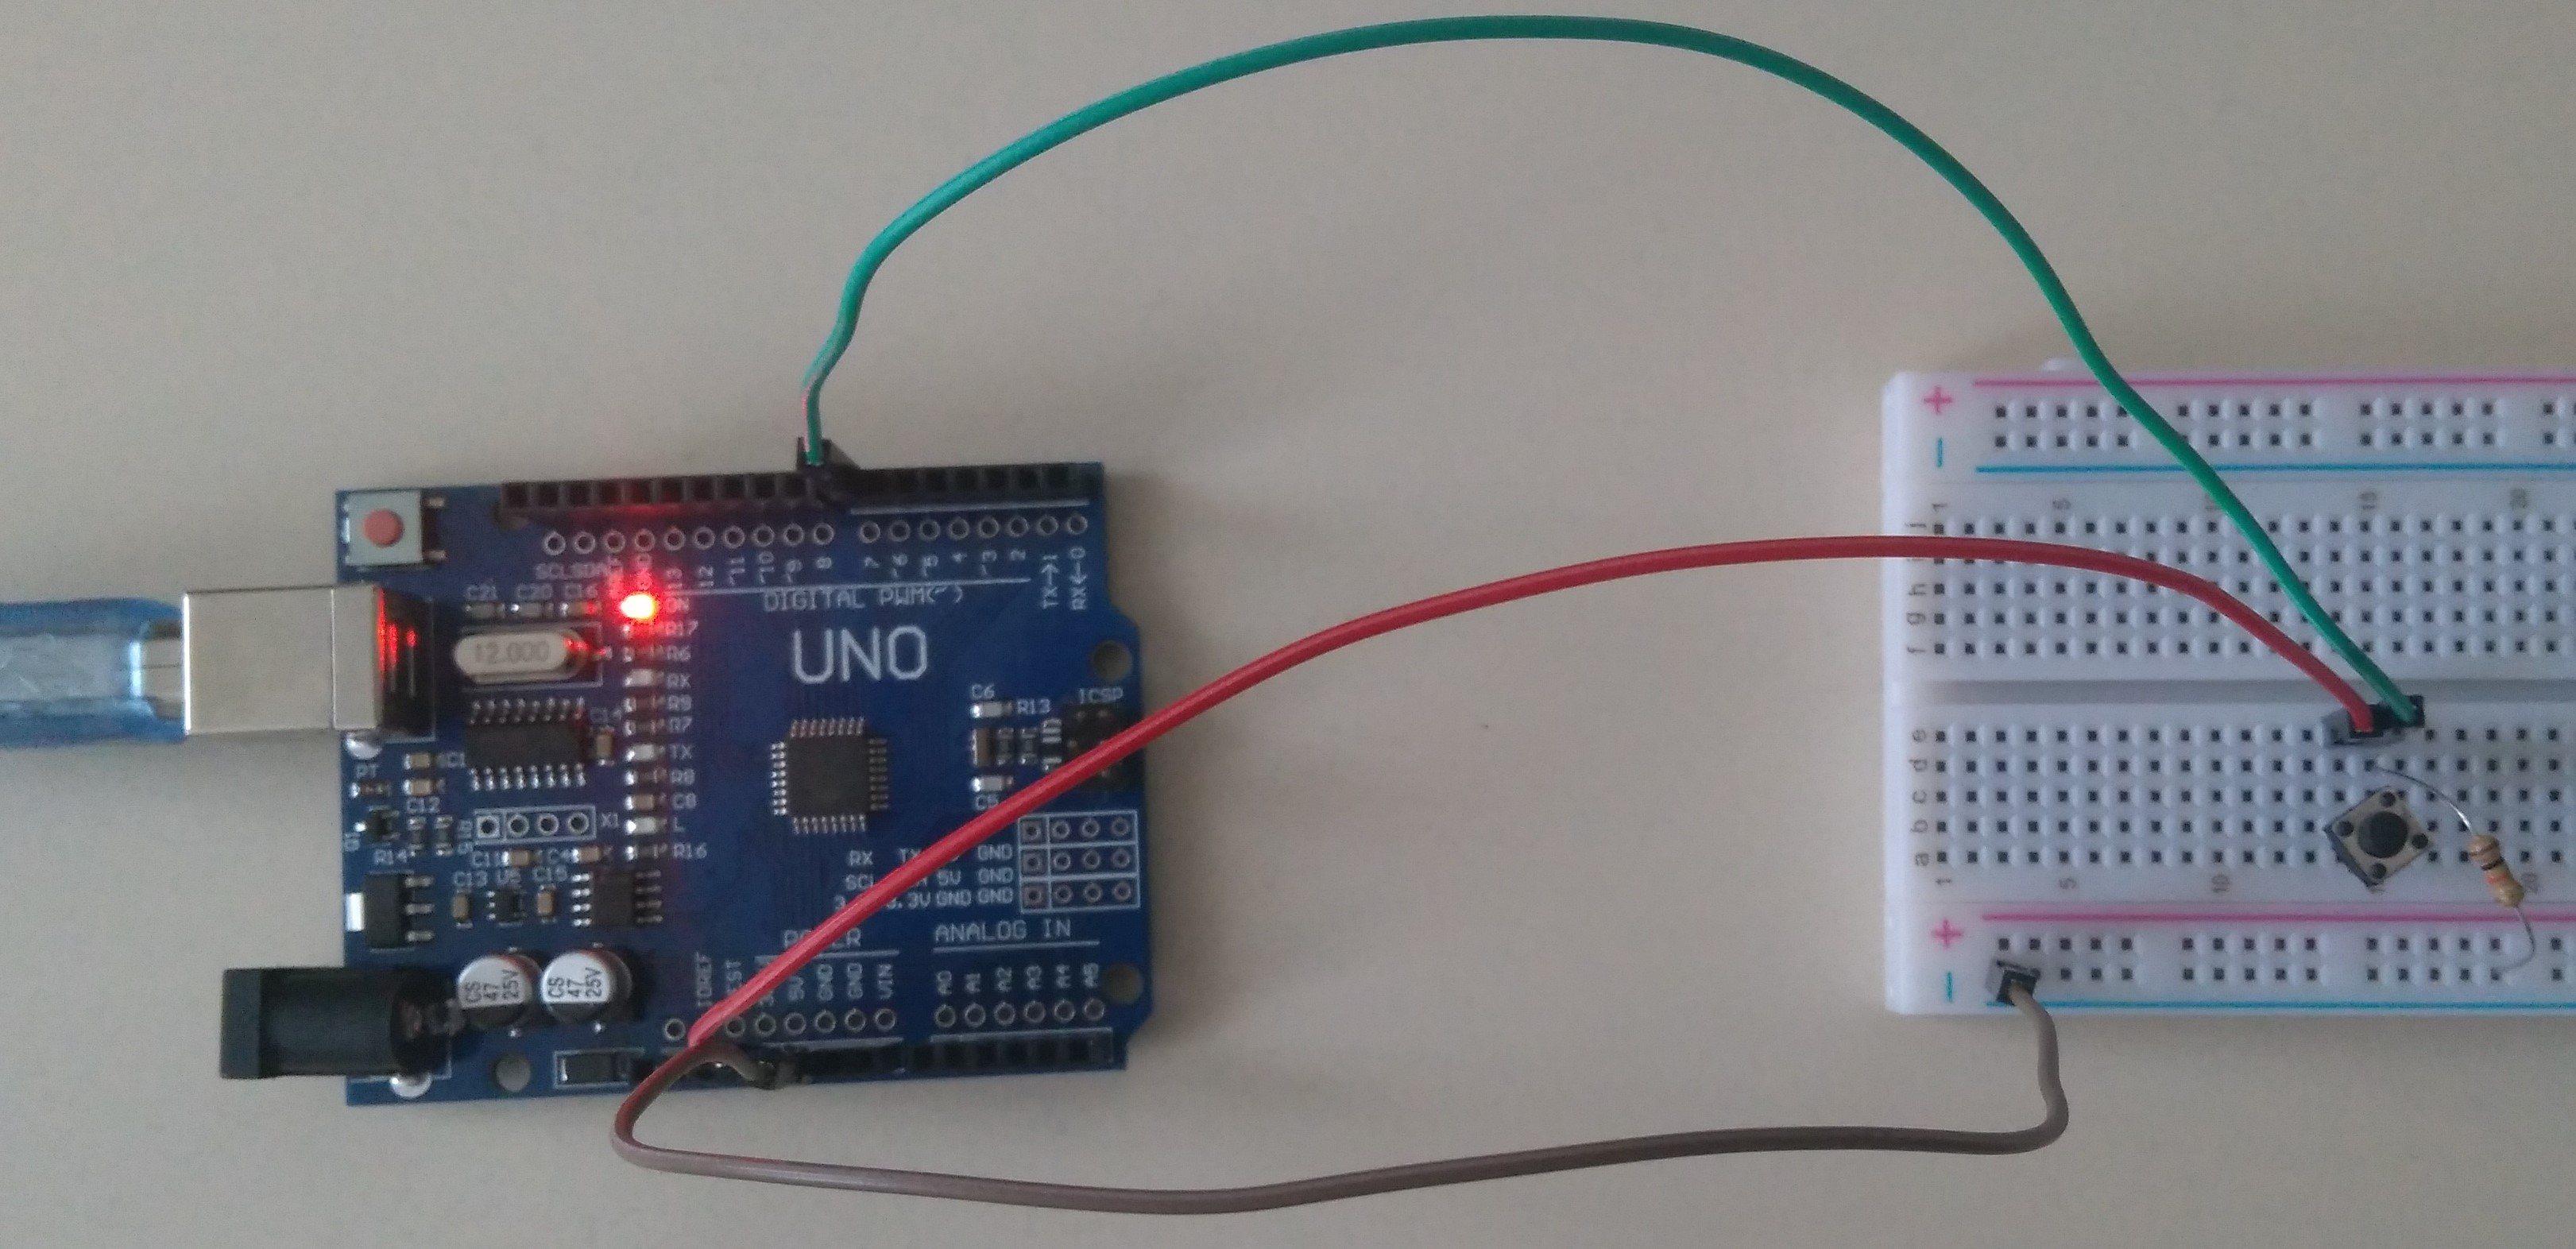
\includegraphics[width=8cm]{idle.jpg}
\end{minipage}
\begin{minipage}{0.5\textwidth}
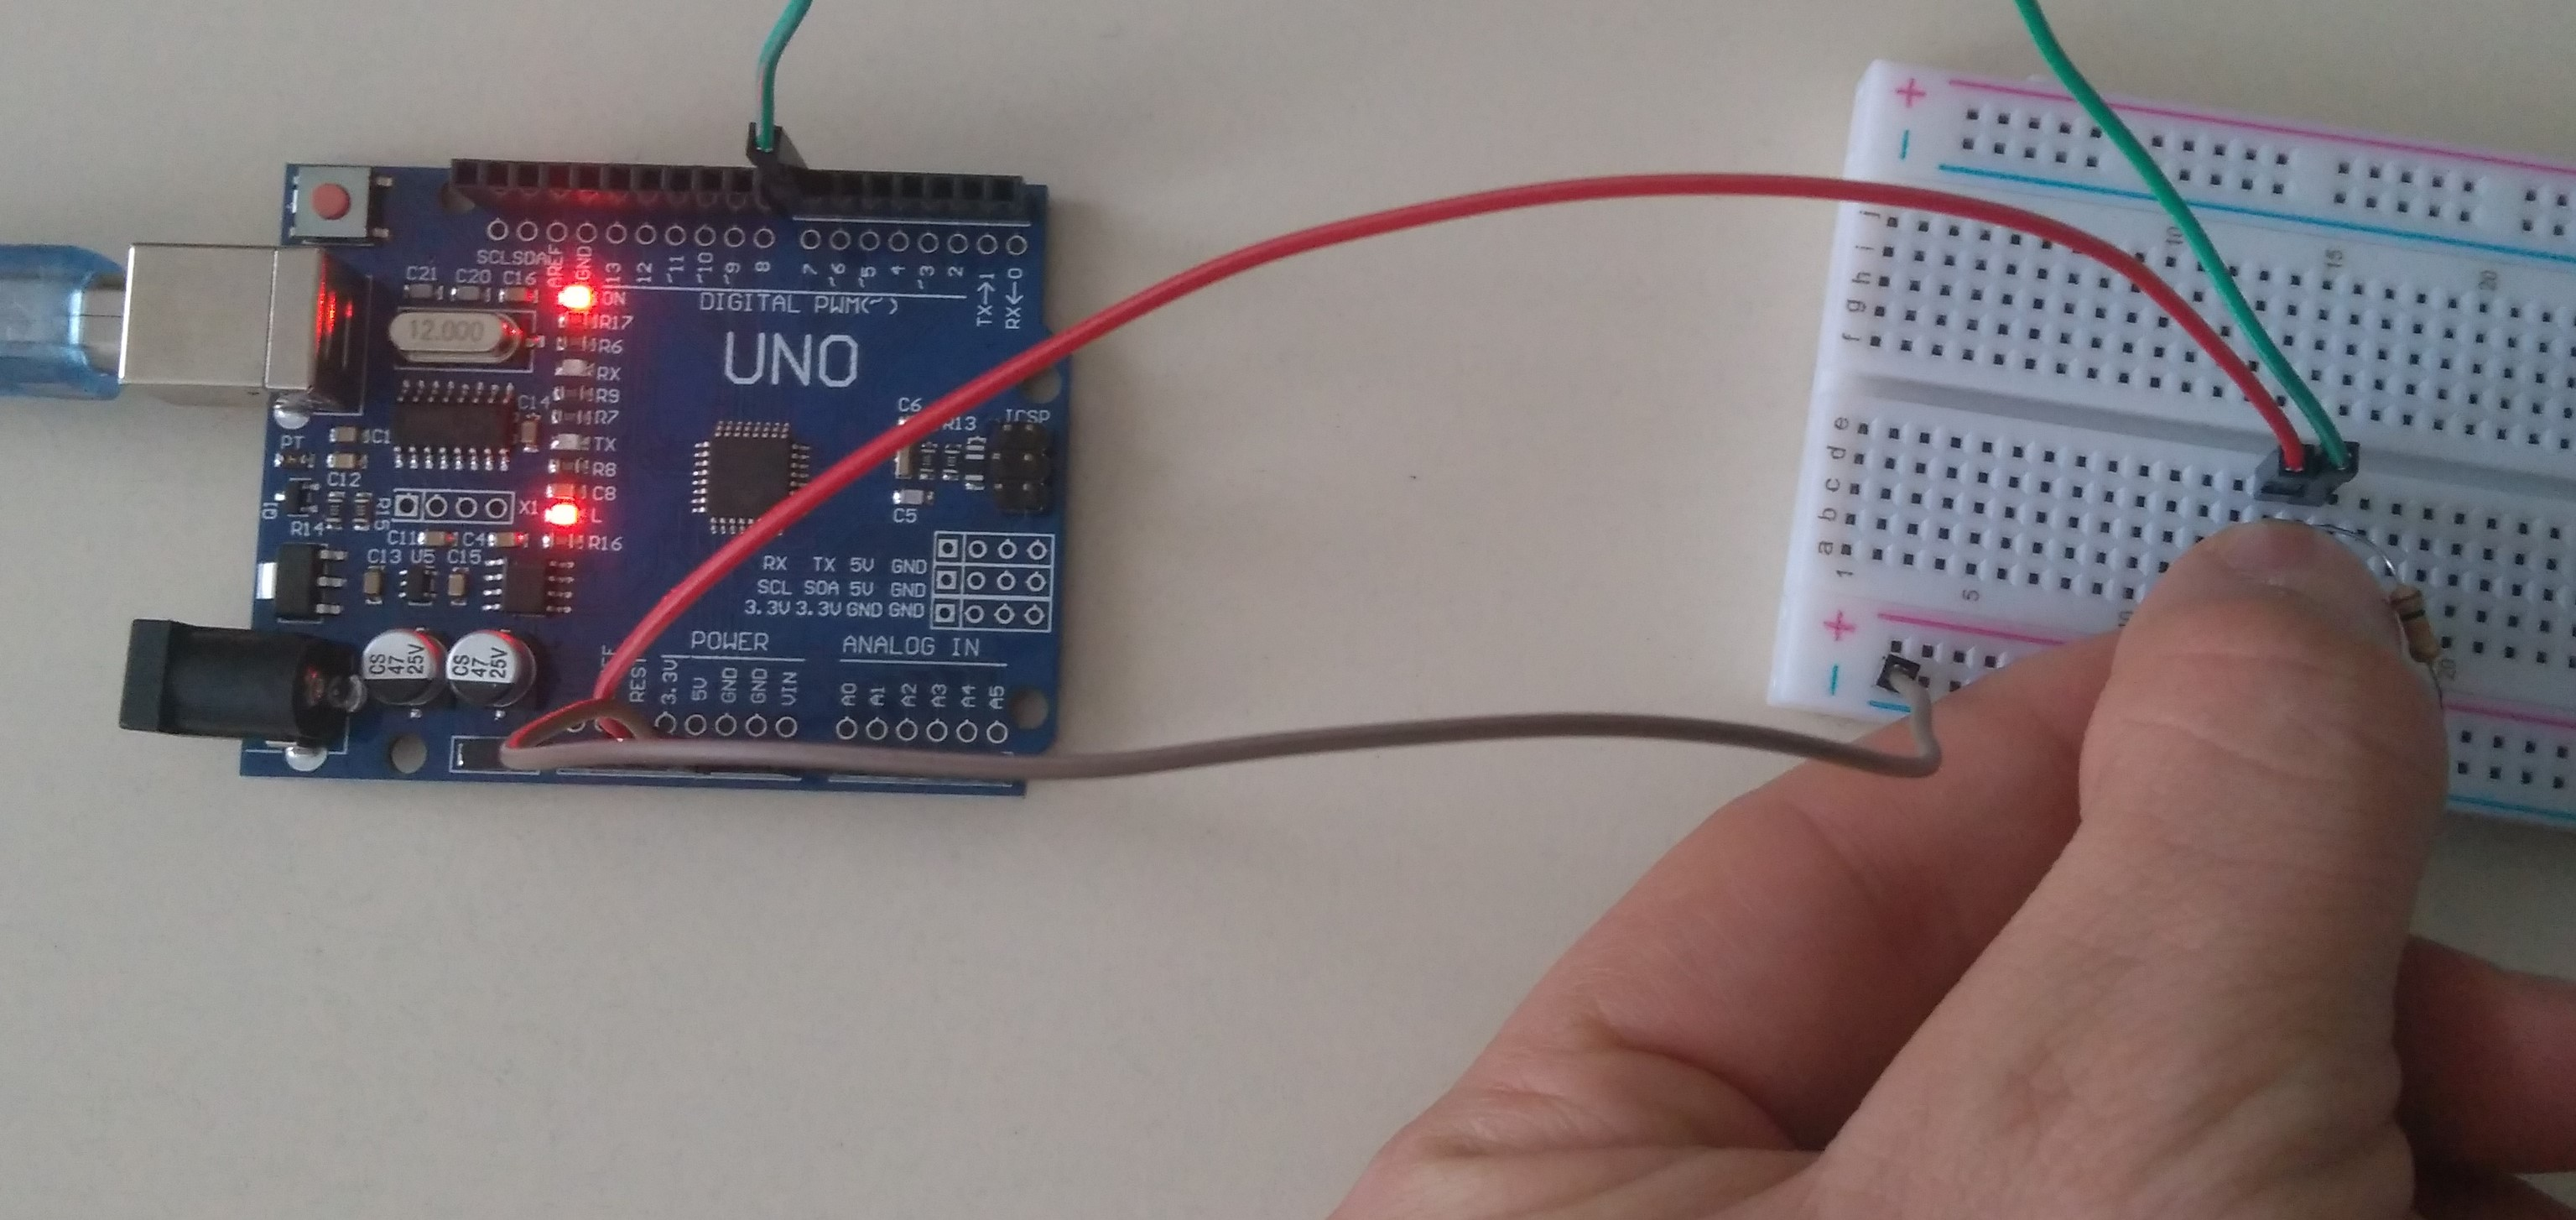
\includegraphics[width=8cm]{pressed.jpg}
\end{minipage}\\

\tab Boşta iken \tab[6cm] Düğmeye basınca\\~\\
Ayrıca Tinkercad sitesinde kod ile birlikte tasarımı görebilirsiniz. Hatta simule de edebilirsiniz.\\
Link(maalesef geçici süreli bir link):
\begin{lstlisting}
https://www.tinkercad.com/things/5QbFNuc1YTu-switch-debouncing
/editel?sharecode=Sg2eclkPXqnJfss5dgNTNYTtQFHs6_j9bT_-jt548DY
\end{lstlisting}
\end{document}
